
\documentclass[a4paper]{article}
\usepackage[margin=.4in]{geometry}
\usepackage[dvipdfmx]{graphicx,xcolor}
\usepackage{amsmath,amssymb}
\usepackage{ascmac}

\begin{document}

\begin{figure*}[t]
  \begin{center}
    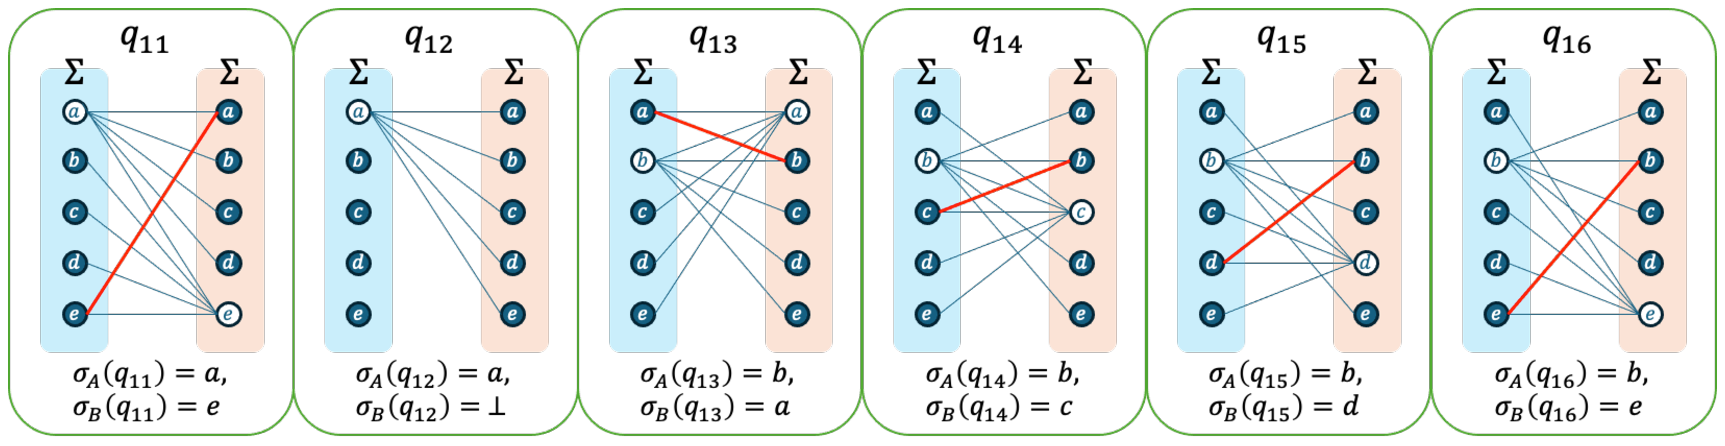
\includegraphics[scale=0.54]{figs/lem11-prop4-eachreg1.pdf}
    \caption{Let $\Sigma=\{a,b,c,d,e\}, Q=\{q_{11},q_{12},q_{13},q_{14},q_{15},q_{16}\}$. From these figures, we get $\ell_A=4$, $\ell_B=1$, $Q^{(\bot,\bot)}=Q^{(\bot,\cdot)}=\emptyset, Q^{(\cdot,\bot)}=\{q_{12}\}$, and $Q^{(\cdot,\cdot)}=\{q_{11},q_{13},q_{14},q_{15},q_{16}\}$. From Proposition~\ref{prop:bothsides}, we note again that for example, even if $p \{ x:=cb \} \preceq q_{14}$ holds, it does not imply that $p \{ x:=xy \} \preceq q_{14}$.}\label{fig:lem11-prop4-eachreg1}
  \end{center}
\end{figure*}

\begin{figure}[t]
  \begin{center}
    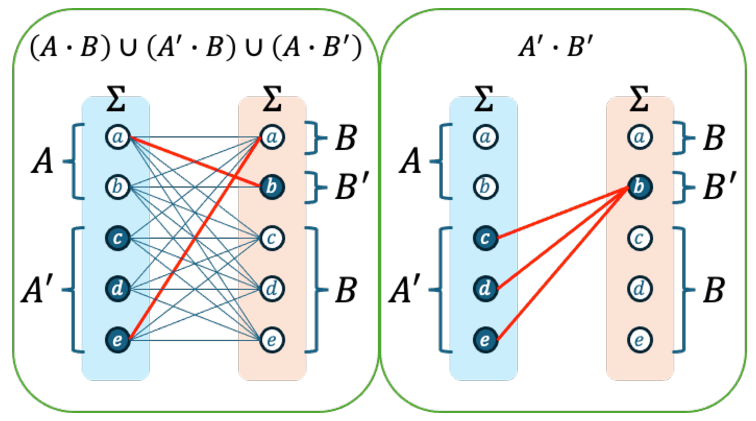
\includegraphics[scale=0.525]{figs/lem11-prop4-totalreg1.pdf}
      \caption{In the left and right figures, we aggregate all of the edges corresponding to $(A\cdot B)\cup (A'\cdot B)\cup (A\cdot B')$ and $A'\cdot B'$ in Fig.~\ref{fig:lem11-prop4-eachreg1}, respectively. From these figures, we get $Q_{1}^{(\cdot,\cdot)}=\{q_{11},q_{13}\}$ and $Q_{2}^{(\cdot,\cdot)}=\{q_{14},q_{15},q_{16}\}$. Then, ${\cal L}_{1}=0$ and ${\cal L}_{2} = 3 \leq \min\{\sharp A' + \ell_B, \sharp B' + \ell_A\} = 4$ holds.}\label{fig:lem11-prop4-totalreg1}
  \end{center}
\end{figure}

\centering{Example 1}

\newpage

\begin{figure*}[t]
  \begin{center}
    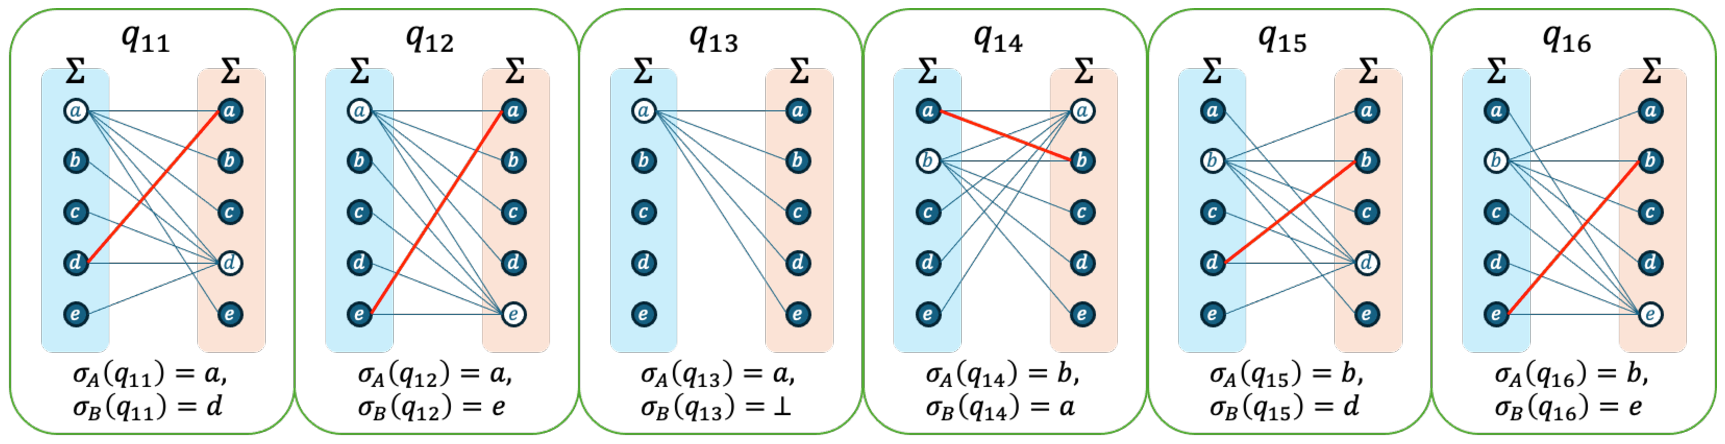
\includegraphics[scale=0.54]{figs/lem11-prop4-eachreg2.pdf}
    \caption{Let $\Sigma=\{a,b,c,d,e\}, Q=\{q_{11},q_{12},q_{13},q_{14},q_{15},q_{16}\}$. From these figures, we get $\ell_A=4$, $\ell_B=1$, $Q^{(\bot,\bot)}=Q^{(\bot,\cdot)}=\emptyset, Q^{(\cdot,\bot)}=\{q_{13}\}$, and $Q^{(\cdot,\cdot)}=\{q_{11},q_{12},q_{14},q_{15},q_{16}\}$. From Proposition~\ref{prop:bothsides}, we note again that for example, even if $p \{ x:=db \} \preceq q_{15}$ holds, it does not imply that $p \{ x:=xy \} \preceq q_{15}$.}\label{fig:lem11-prop4-eachreg2}
  \end{center}
\end{figure*}

\begin{figure}[t]
  \begin{center}
    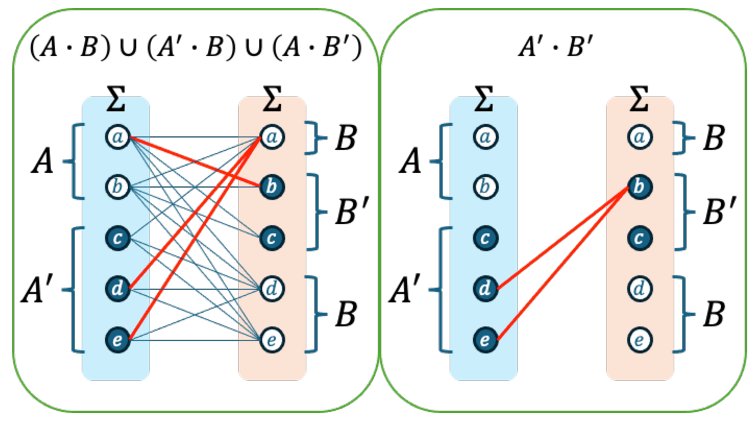
\includegraphics[scale=0.525]{figs/lem11-prop4-totalreg2.pdf}
    \caption{In the left and right figures, we aggregate all of the edges corresponding to $(A\cdot B)\cup (A'\cdot B)\cup (A\cdot B')$ and $A'\cdot B'$ in Fig.~\ref{fig:lem11-prop4-eachreg2}, respectively. From these figures, we get $Q_{1}^{(\cdot,\cdot)}=\{q_{11},q_{12},q_{14}\}$ and $Q_{2}^{(\cdot,\cdot)}=\{q_{15},q_{16}\}$. Then, ${\cal L}_{1} = 0$ and ${\cal L}_{2} = 2 \leq \min\{\sharp A' + \ell_B, \sharp B' + \ell_A\} = 4$ holds.}\label{fig:lem11-prop4-totalreg2}
  \end{center}
\end{figure}

\centering{Example 2}

\newpage

\begin{figure*}[t]
  \begin{center}
    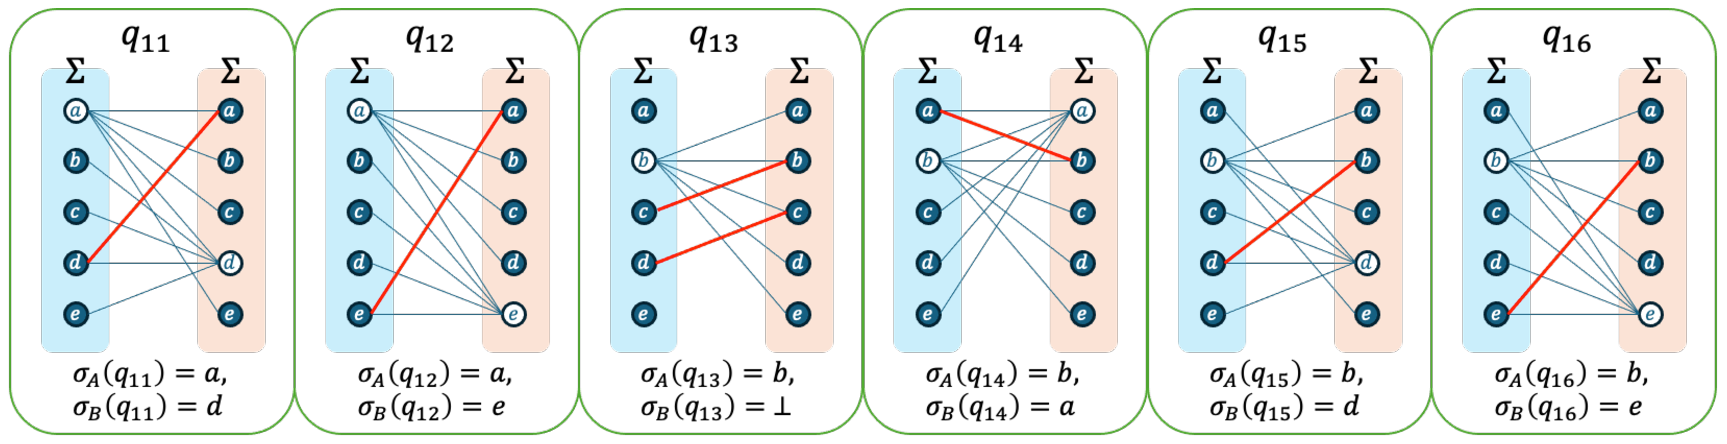
\includegraphics[scale=0.54]{figs/lem11-prop4-eachreg3.pdf}
    \caption{Let $\Sigma=\{a,b,c,d,e\}, Q=\{q_{11},q_{12},q_{13},q_{14},q_{15},q_{16}\}$. From these figures, we get $\ell_A=4$, $\ell_B=1$, $Q^{(\bot,\bot)}=Q^{(\bot,\cdot)}=\emptyset, Q^{(\cdot,\bot)}=\{q_{13}\}$, and $Q^{(\cdot,\cdot)}=\{q_{11},q_{12},q_{14},q_{15},q_{16}\}$. From Proposition~\ref{prop:bothsides}, we note again that for example, even if $p \{ x:=db \} \preceq q_{15}$ holds, it does not imply that $p \{ x:=xy \} \preceq q_{15}$.}\label{fig:lem11-prop4-eachreg2}
  \end{center}
\end{figure*}

\begin{figure}[t]
  \begin{center}
    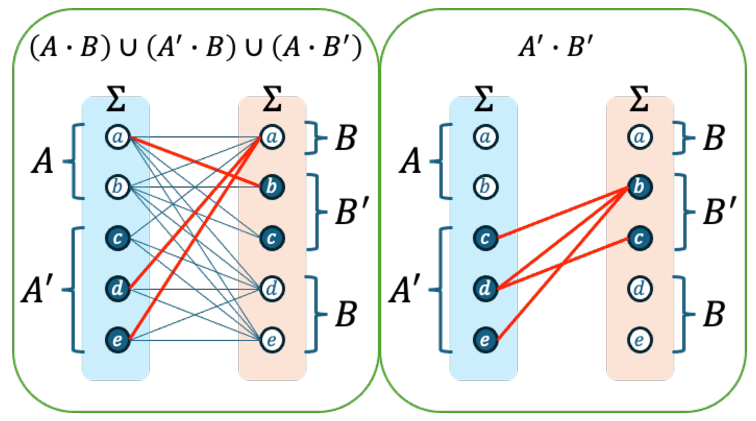
\includegraphics[scale=0.525]{figs/lem11-prop4-totalreg3.pdf}
    \caption{In the left and right figures, we aggregate all of the edges corresponding to $(A\cdot B)\cup (A'\cdot B)\cup (A\cdot B')$ and $A'\cdot B'$ in Fig.~\ref{fig:lem11-prop4-eachreg2}, respectively. From these figures, we get $Q_{1}^{(\cdot,\cdot)}=\{q_{11},q_{12},q_{14}\}$ and $Q_{2}^{(\cdot,\cdot)}=\{q_{15},q_{16}\}$. Then, ${\cal L}_{1} = 2$ and ${\cal L}_{2} = 2 \leq \min\{\sharp A' + \ell_B, \sharp B' + \ell_A\} = 4$ holds.}\label{fig:lem11-prop4-totalreg2}
  \end{center}
\end{figure}

\centering{Example 3}
\end{document}
